% ==============================================================================
%  MIVA-KNIGHT Month 1 — Complete Technical Documentation
%  Multi-modal Industrial Voice Assistant — Knowledge-Integrated Hybrid Retrieval
%  Student: Kayode (Oluwakayode) Soyinka | IT 581 Capstone Project
% ==============================================================================
\documentclass[12pt, a4paper]{article}

% ── Core typesetting ──────────────────────────────────────────────────────────
\usepackage[utf8]{inputenc}
\usepackage[T1]{fontenc}
\usepackage[margin=2.5cm, top=3cm, bottom=3cm]{geometry}

% ── Mathematics ───────────────────────────────────────────────────────────────
\usepackage{amsmath, amssymb, amsthm, mathtools}
\usepackage{bm}

% ── Algorithms ────────────────────────────────────────────────────────────────
\usepackage{algorithm}
\usepackage{algpseudocode}
\algnewcommand\algorithmicinput{\textbf{Input:}}
\algnewcommand\algorithmicoutput{\textbf{Output:}}
\algnewcommand\INPUT{\item[\algorithmicinput]}
\algnewcommand\OUTPUT{\item[\algorithmicoutput]}
\renewcommand{\algorithmiccomment}[1]{\hfill\textit{// #1}}

% ── Graphics & TikZ ───────────────────────────────────────────────────────────
\usepackage{tikz}
\usetikzlibrary{
  shapes.geometric, shapes.misc,
  arrows.meta, arrows,
  positioning, calc, fit,
  backgrounds, shadows.blur,
  decorations.pathreplacing,
  patterns, matrix
}
\usepackage{pgfplots}
\pgfplotsset{compat=1.18}

% ── Tables & Boxes ────────────────────────────────────────────────────────────
\usepackage{booktabs, array, tabularx, multirow}
\usepackage{tcolorbox}
\tcbuselibrary{skins, breakable, theorems}
\usepackage{xcolor}
\usepackage{cancel}
\newcommand{\st}[1]{\cancel{#1}}

% ── Formatting ────────────────────────────────────────────────────────────────
\usepackage{enumitem}
\usepackage{titlesec}
\usepackage{fancyhdr}
\usepackage{hyperref}
\hypersetup{colorlinks=true, linkcolor=NavyBlue, urlcolor=NavyBlue}
\usepackage{graphicx}
\usepackage{float}

% ── Colour palette ────────────────────────────────────────────────────────────
\definecolor{NavyBlue}{RGB}{20,60,120}
\definecolor{CoralRed}{RGB}{210,80,70}
\definecolor{SlateGray}{RGB}{80,100,120}
\definecolor{MintGreen}{RGB}{60,160,110}
\definecolor{Amber}{RGB}{200,140,30}
\definecolor{Lavender}{RGB}{130,100,180}
\definecolor{DeepTeal}{RGB}{20,100,100}
\definecolor{BoxBlue}{RGB}{210,225,245}
\definecolor{BoxRed}{RGB}{245,215,215}
\definecolor{BoxOrange}{RGB}{255,232,205}
\definecolor{BoxGray}{RGB}{228,228,228}
\definecolor{BoxGreen}{RGB}{205,235,215}
\definecolor{BoxPurple}{RGB}{230,215,245}
\definecolor{DarkContainer}{RGB}{195,210,232}

% ── Theorem environments ──────────────────────────────────────────────────────
\theoremstyle{definition}
\newtheorem{definition}{Definition}[section]
\newtheorem{axiom}{Axiom}[section]

\theoremstyle{plain}
\newtheorem{theorem}{Theorem}[section]
\newtheorem{lemma}{Lemma}[section]
\newtheorem{corollary}{Corollary}[section]
\newtheorem{proposition}{Proposition}[section]

\theoremstyle{remark}
\newtheorem{remark}{Remark}[section]
\newtheorem{example}{Example}[section]

% ── tcolorbox styles ──────────────────────────────────────────────────────────
\tcbset{
  layman/.style={
    enhanced, breakable,
    colback=BoxOrange!50, colframe=Amber!80,
    fonttitle=\bfseries\small,
    title={Simple Explanation (Non-technical)},
    left=5pt, right=5pt, top=5pt, bottom=5pt,
    before skip=6pt, after skip=6pt
  },
  notebox/.style={
    enhanced, breakable,
    colback=BoxGreen!50, colframe=MintGreen!80,
    fonttitle=\bfseries\small,
    left=5pt, right=5pt, top=5pt, bottom=5pt,
    before skip=4pt, after skip=4pt
  }
}

% ── Page style ────────────────────────────────────────────────────────────────
\pagestyle{fancy}
\fancyhf{}
\fancyhead[L]{\small\textcolor{NavyBlue}{MIVA-KNIGHT Month 1 --- Technical Documentation}}
\fancyhead[R]{\small\textcolor{NavyBlue}{IT 581 --- Kayode Soyinka}}
\fancyfoot[C]{\thepage}
\renewcommand{\headrulewidth}{0.4pt}

% ── Section formatting ────────────────────────────────────────────────────────
\titleformat{\section}[block]
  {\large\bfseries\color{NavyBlue}}{\thesection}{1em}{}[\titlerule]
\titleformat{\subsection}[block]
  {\normalsize\bfseries\color{SlateGray}}{\thesubsection}{1em}{}
\titleformat{\subsubsection}[runin]
  {\normalsize\bfseries\color{DeepTeal}}{\thesubsubsection}{0.5em}{\ }[.]

% ── TikZ node styles (matching GCN reference) ─────────────────────────────────
\tikzset{
  basebox/.style={rectangle, rounded corners=4pt, draw=black!55,
    align=center, font=\small},
  databox/.style={basebox, fill=black!85, text=white,
    minimum width=2.4cm, minimum height=1.5cm},
  procbox/.style={basebox, fill=BoxBlue, thick,
    minimum width=3.0cm, minimum height=1.3cm},
  lossbox/.style={basebox, fill=BoxRed,
    minimum width=3.2cm, minimum height=1.2cm},
  trainbox/.style={basebox, fill=BoxOrange, thick,
    minimum width=3.4cm, minimum height=1.2cm},
  inferbox/.style={basebox, fill=BoxGreen,
    minimum width=3.2cm, minimum height=1.2cm},
  kgbox/.style={basebox, fill=BoxPurple,
    minimum width=3.2cm, minimum height=1.4cm},
  outputbox/.style={basebox, fill=BoxGray,
    minimum width=3.2cm, minimum height=1.2cm},
  arrow/.style={->, >=Stealth, thick, color=black!70},
  thickarrow/.style={->, >=Stealth, very thick, color=black},
  redarrow/.style={->, >=Stealth, thick, color=CoralRed!80},
  greenarrow/.style={->, >=Stealth, thick, color=MintGreen!80},
  purplearrow/.style={->, >=Stealth, thick, color=Lavender!80},
  dasharrow/.style={->, >=Stealth, thick, dashed, color=black!50}
}

% ==============================================================================
\begin{document}
% ==============================================================================

% ─── TITLE PAGE ───────────────────────────────────────────────────────────────
\begin{titlepage}
  \centering
  \vspace*{1.5cm}

  {\Huge\bfseries\color{NavyBlue} MIVA-KNIGHT}\\[0.5cm]
  {\Large\color{SlateGray} Multi-modal Industrial Voice Assistant}\\[0.2cm]
  {\Large\color{SlateGray} Knowledge-Integrated Hybrid Retrieval}\\[1.2cm]

  \begin{tcolorbox}[notebox, width=0.88\textwidth,
      title={Month 1 Complete Technical Documentation}]
    \centering
    \textbf{Text + Image Fusion with Knowledge-Graph-Boosted Hybrid Retrieval}\\[0.4cm]
    This document provides the complete mathematical derivation, formal
    algorithm specifications, theorems, lemmas, axioms, pseudocode, TikZ
    figures, and full pipeline flowchart for the Month~1 MIVA-KNIGHT
    implementation.  Every algorithm is explained in both rigorous technical
    terms and accessible layman language.
  \end{tcolorbox}

  \vspace{1.2cm}
  \begin{tabular}{@{}ll}
    \textbf{Student:} & Kayode (Oluwakayode) Soyinka \\[2pt]
    \textbf{Course:}  & IT 581 --- Capstone Project \\[2pt]
    \textbf{Month:}   & 1 of 6 \\[2pt]
    \textbf{Dataset:} & COCO val2017 ($\sim$5\,000 images, 5 captions each) \\[2pt]
    \textbf{Hardware:}& Google Colab T4 GPU (15\,GB VRAM) \\[2pt]
    \textbf{Runtime:} & $\sim$10--15 min on GPU $\cdot$ $\sim$30--60 min on CPU \\
  \end{tabular}

  \vspace{2cm}
  \tableofcontents
\end{titlepage}

% ==============================================================================
\section{System Overview and Design Principles}
% ==============================================================================

\subsection{What MIVA-KNIGHT Builds}

MIVA-KNIGHT is a \emph{multi-modal retrieval and fusion} system that learns
joint representations from four data streams: text, images, voice, and sensor
data.  Month~1 establishes the foundational architecture using only
\textbf{text and images}, building every component that Months~2--6 extend.

\begin{tcolorbox}[layman]
Imagine a very smart research assistant who can understand both written
descriptions and photographs.  You show them a photo of a dog running on a
beach and they instantly search thousands of image-caption pairs to find all
entries about dogs, beaches, and outdoor activities --- even when the exact
words differ.  MIVA-KNIGHT is that assistant.  Month~1 teaches the system
to understand text and images together, building the foundation for voice
and sensor understanding in later months.
\end{tcolorbox}

\subsection{Formal Design Axioms}

\begin{axiom}[Shared Embedding Space]
A shared embedding space $\mathcal{E} \subset \mathbb{R}^d$ exists such that
semantically similar content from \emph{different} modalities projects to
geometrically close points:
\[
  \forall\,(x_m, x_n)\;\text{semantically equivalent}:\quad
  \|f_m(x_m) - f_n(x_n)\|_2 \;\ll\;
  \|f_m(x_m) - f_n(x'_n)\|_2
\]
where $x'_n$ is any semantically unrelated sample from modality $n$.
\end{axiom}

\begin{axiom}[Frozen Backbone Pre-training]
Pre-trained encoder backbones (BERT, ResNet-50) have learned general-purpose
features that transfer effectively to retrieval tasks.  Their weights are
frozen during MIVA-KNIGHT training to preserve these features and reduce the
trainable parameter count from $\sim$138\,M to $\sim$5\,M.
\end{axiom}

\begin{axiom}[Knowledge Graph Co-occurrence]
Two entities $e_1, e_2$ are semantically related if they co-occur in the
same training caption.  This approximates Pointwise Mutual Information (PMI)
as a proxy for semantic relatedness without explicit human annotation.
\end{axiom}

\subsection{Component Summary}

\begin{center}
\renewcommand{\arraystretch}{1.2}
\begin{tabular}{@{}lllr@{}}
\toprule
\textbf{Component} & \textbf{Input} & \textbf{Output Shape} &
\textbf{Trainable Params} \\
\midrule
BERT-base encoder       & Text string           & $\mathbb{R}^{768}$      & 0 (frozen) \\
ResNet-50 backbone      & $[3,224,224]$ tensor  & $\mathbb{R}^{2048}$     & 0 (frozen) \\
Image Projection head   & $\mathbb{R}^{2048}$   & $\mathbb{R}^{768}$      & $\sim$1.57\,M \\
Text Projection head    & $\mathbb{R}^{768}$    & $\mathbb{R}^{512}$      & $\sim$393\,K  \\
MultiModal Fusion       & $4\times\mathbb{R}^{512}$ & $\mathbb{R}^{512}$  & $\sim$3.10\,M \\
Knowledge Graph         & Corpus captions       & Graph $\mathcal{G}$     & N/A \\
Hybrid Retriever        & Query $q$             & Ranked documents        & 0 \\
\midrule
\textbf{Total trainable} & & & $\sim$5.06\,M \\
\textbf{Total frozen}    & & & $\sim$133.5\,M \\
\bottomrule
\end{tabular}
\end{center}

% ==============================================================================
\section{Full Pipeline Flowchart}
\label{sec:flowchart}
% ==============================================================================

Figure~\ref{fig:pipeline} presents the complete Month~1 pipeline in the
same visual style as the GCN reference diagram.  Colour coding:
\textcolor{NavyBlue}{\textbf{blue}} = feature extraction (frozen + trainable projections),
\textcolor{CoralRed}{\textbf{red}} = training and loss,
\textcolor{Lavender}{\textbf{purple}} = knowledge graph and retrieval,
\textcolor{MintGreen}{\textbf{green}} = inference outputs.
Dashed arrows indicate gradient flow during backpropagation.

\begin{figure}[H]
\centering
\resizebox{\textwidth}{!}{%
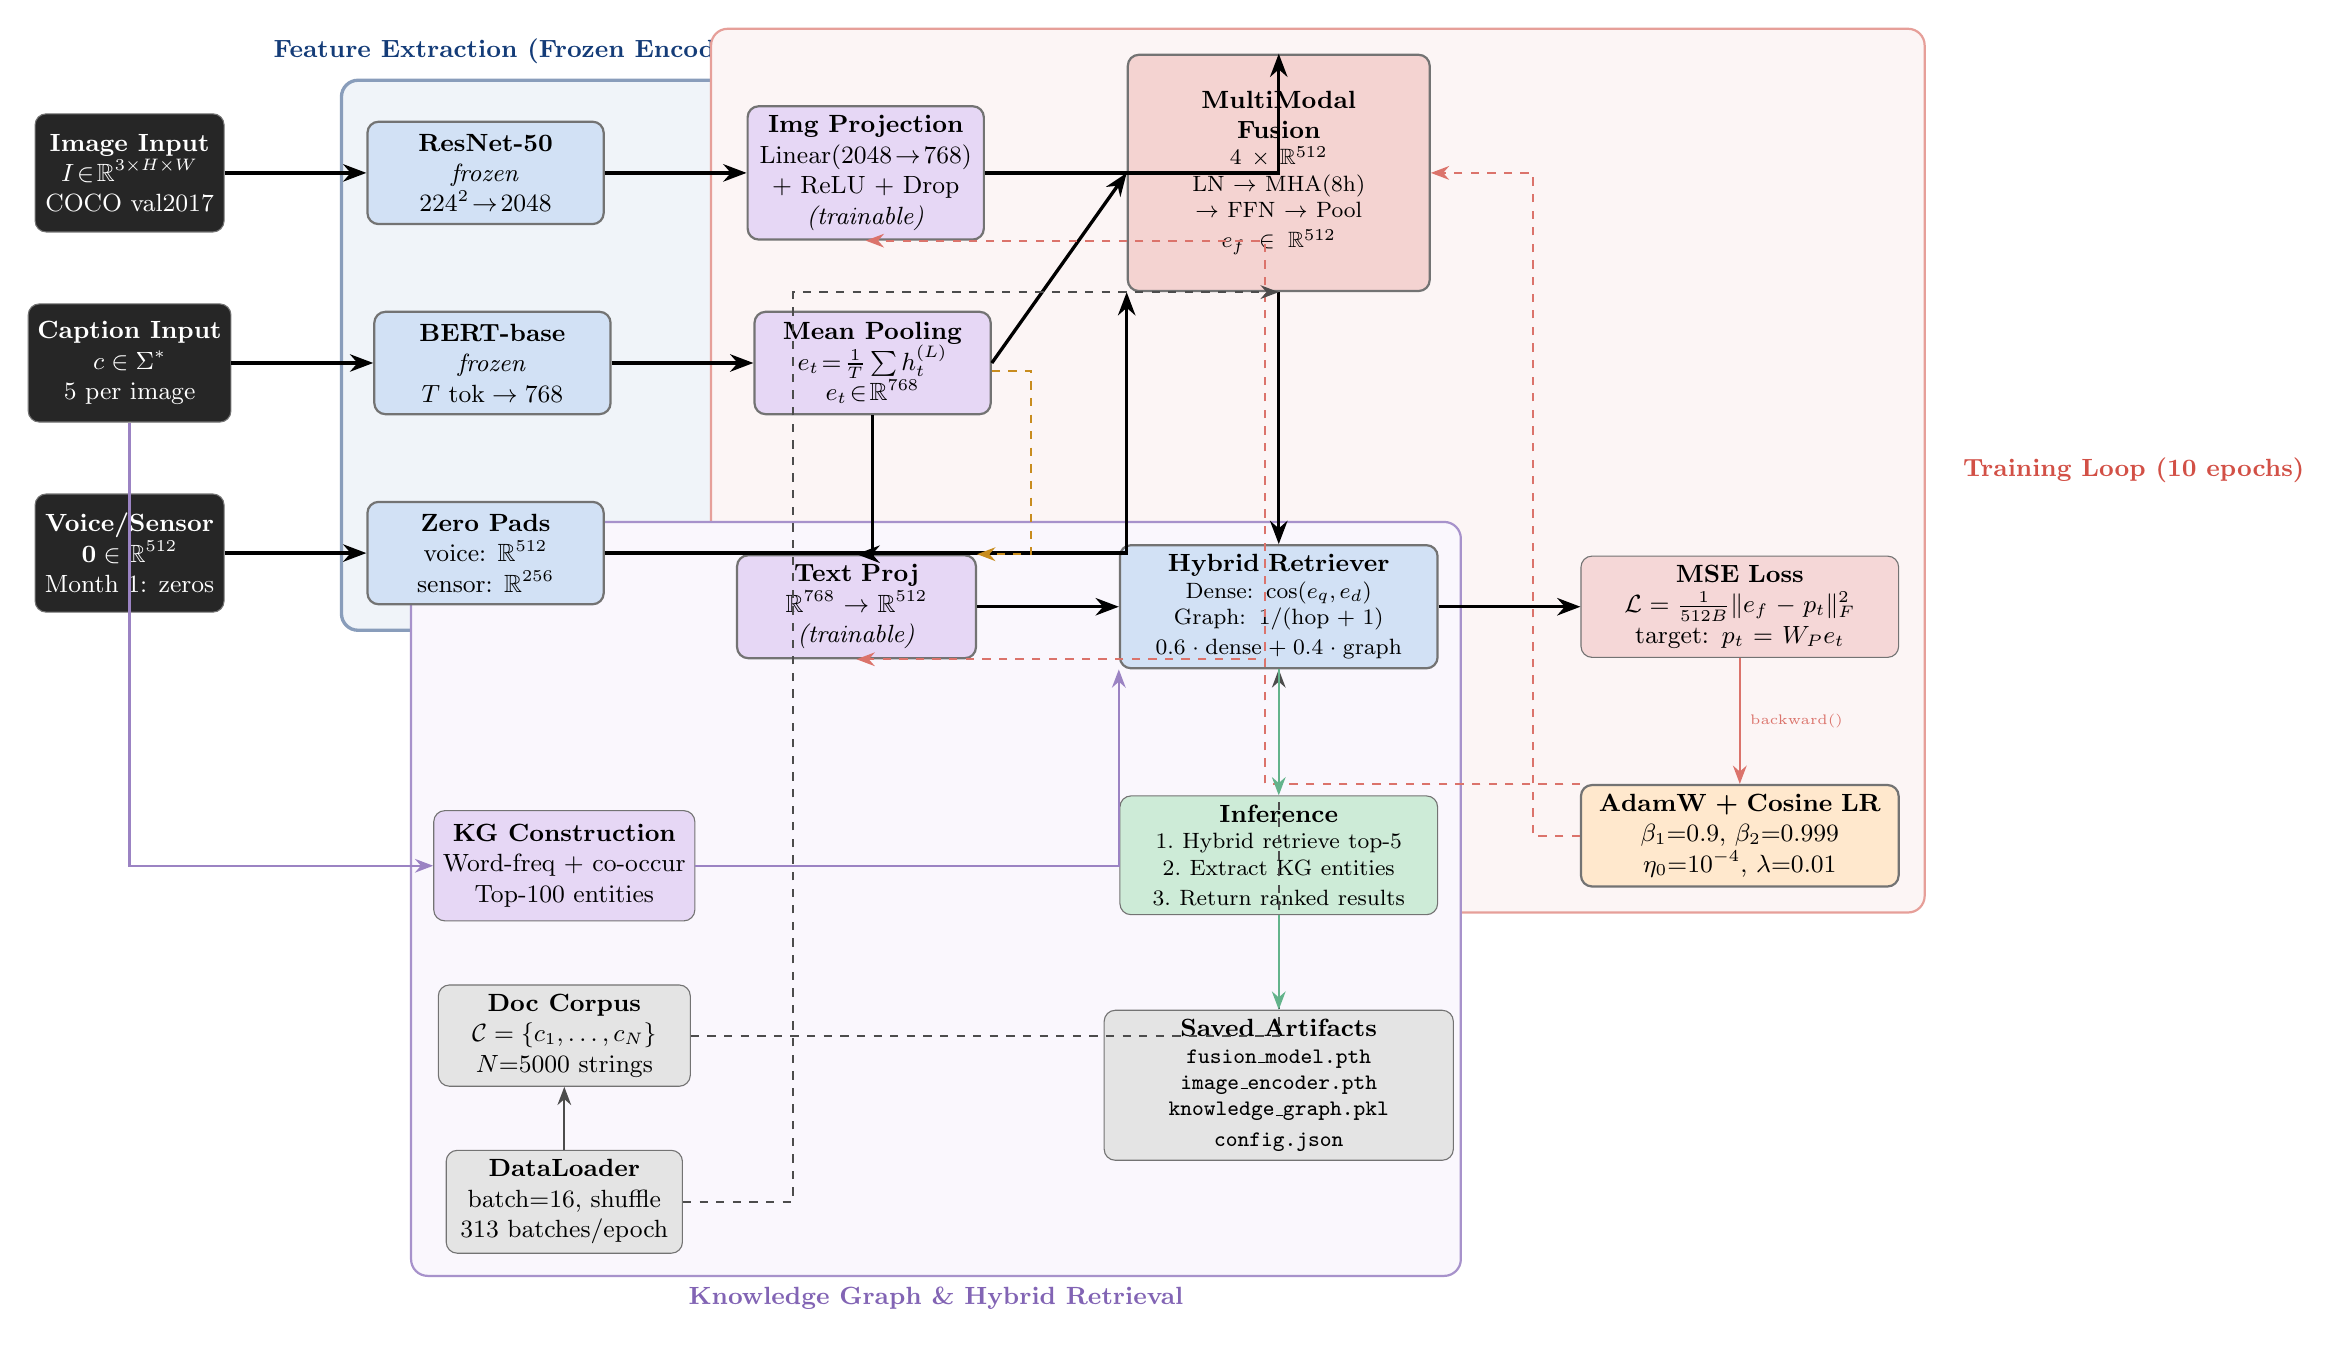
\begin{tikzpicture}[node distance=1.0cm and 1.3cm]

  % ===== COLUMN 0: DATA INPUTS =====
  \node[databox] (imgInput) {
    \textbf{Image Input}\\
    $I\!\in\!\mathbb{R}^{3\times H\times W}$\\
    COCO val2017
  };
  \node[databox, below=0.9cm of imgInput] (txtInput) {
    \textbf{Caption Input}\\
    $c \in \Sigma^*$\\
    5 per image
  };
  \node[databox, below=0.9cm of txtInput] (voiceInput) {
    \textbf{Voice/Sensor}\\
    $\mathbf{0} \in \mathbb{R}^{512}$\\
    Month 1: zeros
  };

  % ===== COLUMN 1: ENCODERS =====
  \node[procbox, right=1.8cm of imgInput] (resnet) {
    \textbf{ResNet-50}\\
    \textit{frozen}\\
    $224^2\!\to\!2048$
  };
  \node[procbox, right=1.8cm of txtInput] (bert) {
    \textbf{BERT-base}\\
    \textit{frozen}\\
    $T\text{ tok}\to 768$
  };
  \node[procbox, right=1.8cm of voiceInput] (zeropad) {
    \textbf{Zero Pads}\\
    voice: $\mathbb{R}^{512}$\\
    sensor: $\mathbb{R}^{256}$
  };

  % ===== COLUMN 2: PROJECTIONS =====
  \node[procbox, right=1.8cm of resnet, fill=BoxPurple] (imgproj) {
    \textbf{Img Projection}\\
    Linear$(2048\!\to\!768)$\\
    + ReLU + Drop\\
    \textit{(trainable)}
  };
  \node[procbox, right=1.8cm of bert, fill=BoxPurple] (meanpool) {
    \textbf{Mean Pooling}\\
    $e_t\!=\!\frac{1}{T}\sum h_t^{(L)}$\\
    $e_t\!\in\!\mathbb{R}^{768}$
  };

  % ===== KG BOX (sits below encoders) =====
  \node[kgbox, below=2.6cm of zeropad, xshift=1.0cm] (kgbuild) {
    \textbf{KG Construction}\\
    Word-freq + co-occur\\
    Top-100 entities
  };

  % ===== FUSION BOX =====
  \node[procbox, right=1.8cm of imgproj, fill=CoralRed!25,
        minimum height=3.0cm, text width=3.6cm] (fusion) {
    \textbf{MultiModal}\\
    \textbf{Fusion}\\
    \footnotesize
    $4\times\mathbb{R}^{512}$\\
    LN $\to$ MHA(8h)\\
    $\to$ FFN $\to$ Pool\\
    $e_f\!\in\!\mathbb{R}^{512}$
  };

  % ===== DOCUMENT CORPUS =====
  \node[outputbox, below=0.8cm of kgbuild] (corpus) {
    \textbf{Doc Corpus}\\
    $\mathcal{C}=\{c_1,\ldots,c_N\}$\\
    $N{=}5000$ strings
  };

  % ===== DATALOADER =====
  \node[basebox, fill=BoxGray, below=0.8cm of corpus, minimum width=3.0cm] (loader) {
    \textbf{DataLoader}\\
    batch=16, shuffle\\
    313 batches/epoch
  };

  % ===== HYBRID RETRIEVER =====
  \node[procbox, below=3.2cm of fusion, fill=BoxBlue, text width=3.8cm] (retriever) {
    \textbf{Hybrid Retriever}\\
    \footnotesize
    Dense: $\cos(e_q, e_d)$\\
    Graph: $1/(\text{hop}+1)$\\
    $0.6\cdot\text{dense}+0.4\cdot\text{graph}$
  };

  % ===== TEXT PROJECTION =====
  \node[procbox, left=1.8cm of retriever, fill=BoxPurple, text width=2.8cm] (txtproj) {
    \textbf{Text Proj}\\
    $\mathbb{R}^{768}\!\to\!\mathbb{R}^{512}$\\
    \textit{(trainable)}
  };

  % ===== LOSS =====
  \node[lossbox, right=1.8cm of retriever, text width=3.8cm] (loss) {
    \textbf{MSE Loss}\\
    $\mathcal{L}\!=\!\frac{1}{512B}\|e_f - p_t\|_F^2$\\
    target: $p_t\!=\!W_P e_t$
  };

  % ===== ADAMW =====
  \node[trainbox, below=1.6cm of loss, text width=3.8cm] (adamw) {
    \textbf{AdamW + Cosine LR}\\
    $\beta_1{=}0.9$, $\beta_2{=}0.999$\\
    $\eta_0{=}10^{-4}$, $\lambda{=}0.01$
  };

  % ===== INFERENCE =====
  \node[inferbox, below=1.6cm of retriever, text width=3.8cm] (inference) {
    \textbf{Inference}\\
    \footnotesize
    1.~Hybrid retrieve top-5\\
    2.~Extract KG entities\\
    3.~Return ranked results
  };

  % ===== OUTPUT ARTIFACTS =====
  \node[outputbox, below=1.2cm of inference, text width=4.2cm] (output) {
    \textbf{Saved Artifacts}\\
    \footnotesize
    \texttt{fusion\_model.pth}\\
    \texttt{image\_encoder.pth}\\
    \texttt{knowledge\_graph.pkl}\\
    \texttt{config.json}
  };

  % ===== ARROWS =====

  % Inputs to encoders
  \draw[thickarrow] (imgInput.east) -- (resnet.west);
  \draw[thickarrow] (txtInput.east) -- (bert.west);
  \draw[thickarrow] (voiceInput.east) -- (zeropad.west);

  % Encoders to projections
  \draw[thickarrow] (resnet.east) -- (imgproj.west);
  \draw[thickarrow] (bert.east) -- (meanpool.west);

  % Projections to fusion
  \draw[thickarrow] (imgproj.east) -| (fusion.north);
  \draw[thickarrow] (meanpool.east) -- (fusion.west);
  \draw[thickarrow] (zeropad.east) -| (fusion.south west);

  % Fusion to retriever and loss
  \draw[thickarrow] (fusion.south) -- (retriever.north);
  \draw[thickarrow] (meanpool.south) |- (txtproj.north);
  \draw[thickarrow] (txtproj.east) -- (retriever.west);
  \draw[thickarrow] (retriever.east) -- (loss.west);

  % Loss backward arrows
  \draw[redarrow] (loss.south) -- node[right, font=\tiny]{backward()} (adamw.north);
  \draw[redarrow, dashed] (adamw.west) -| ++(-0.6, 0) |- (fusion.east);
  \draw[redarrow, dashed] (adamw.north west) -- ++(-4.0,0) |- (imgproj.south);
  \draw[redarrow, dashed] (adamw.north west) -- ++(-4.0,0) |- (txtproj.south);

  % KG connections
  \draw[purplearrow] (txtInput.south) |- (kgbuild.west);
  \draw[purplearrow] (kgbuild.east) -| (retriever.south west);

  % DataLoader & corpus
  \draw[arrow] (loader.north) -- (corpus.south);
  \draw[arrow, dashed] (corpus.east) -| (retriever.south);
  \draw[arrow, dashed] (loader.east) -- ++(1.4,0) |- (fusion.south);

  % Inference chain
  \draw[greenarrow] (retriever.south) -- (inference.north);
  \draw[greenarrow] (inference.south) -- (output.north);

  % Text branch to loss target
  \draw[arrow, Amber, dashed] (meanpool.east) ++(0,-0.1) -- ++(0.5,0) |- (txtproj.north east);

  % ===== BACKGROUND CONTAINERS =====
  \begin{pgfonlayer}{background}
    \node[rectangle, draw=NavyBlue!50, fill=DarkContainer!25,
          rounded corners=6pt, very thick,
          fit=(resnet)(bert)(zeropad)(imgproj)(meanpool),
          inner sep=9pt,
          label={[font=\small\bfseries, color=NavyBlue, yshift=2pt]above:%
                 Feature Extraction (Frozen Encoders + Trainable Projections)}] {};

    \node[rectangle, draw=CoralRed!55, fill=BoxRed!25,
          rounded corners=6pt, thick,
          fit=(fusion)(loss)(adamw)(txtproj),
          inner sep=9pt,
          label={[font=\small\bfseries, color=CoralRed, xshift=10pt]right:%
                 Training Loop (10 epochs)}] {};

    \node[rectangle, draw=Lavender!70, fill=BoxPurple!20,
          rounded corners=6pt, thick,
          fit=(kgbuild)(corpus)(loader)(retriever),
          inner sep=8pt,
          label={[font=\small\bfseries, color=Lavender]below:%
                 Knowledge Graph \& Hybrid Retrieval}] {};
  \end{pgfonlayer}

\end{tikzpicture}
}% end resizebox
\caption{MIVA-KNIGHT Month~1 --- Full System Pipeline.
  \textcolor{NavyBlue}{\textbf{Blue}} = feature extraction.
  \textcolor{CoralRed}{\textbf{Red}} = training / loss.
  \textcolor{Lavender}{\textbf{Purple}} = knowledge graph / retrieval.
  \textcolor{MintGreen}{\textbf{Green}} = inference path.
  Dashed arrows = gradient flow during backpropagation.}
\label{fig:pipeline}
\end{figure}

% ==============================================================================
\section{Data Pipeline}
\label{sec:data}
% ==============================================================================

\subsection{COCO Dataset Loader}

\begin{definition}[COCO Annotation Map]
Given the JSON annotation file containing images list $\mathcal{I}$ and
annotations list $\mathcal{A}$, the annotation map is:
\[
  \phi : \text{image\_id} \;\longrightarrow\; [a_1, a_2, a_3, a_4, a_5]
\]
implemented as a Python \texttt{defaultdict(list)} built by iterating over
every $(a.\texttt{image\_id},\; a.\texttt{caption})$ pair in $\mathcal{A}$.
\end{definition}

\begin{algorithm}[H]
\caption{COCODataset --- Construction and Item Access}
\label{alg:coco}
\begin{algorithmic}[1]
\INPUT{Image directory \texttt{img\_dir}; annotation JSON \texttt{ann\_file}; optional \texttt{max\_samples}}
\OUTPUT{Indexable dataset yielding \texttt{\{image, caption, image\_id\}}}
\Statex
\Procedure{COCODataset.\_\_init\_\_}{img\_dir, ann\_file, max\_samples}
  \State data $\gets$ \texttt{json.load}(ann\_file)
  \State images $\gets$ $\{\,$img[\texttt{id}]: img $\mid$ img $\in$ data[\texttt{images}]$\,\}$
  \State $\phi \gets$ \texttt{defaultdict(list)}
  \For{$a \in$ data[\texttt{annotations}]}
    \State $\phi[a.\texttt{image\_id}]$.\texttt{append}($a$)
  \EndFor
  \State img\_ids $\gets$ list($\phi$.\texttt{keys}())[:max\_samples]
\EndProcedure
\Statex
\Procedure{COCODataset.\_\_getitem\_\_}{idx}
  \State img\_id $\gets$ img\_ids[idx]
  \State path $\gets$ img\_dir / images[img\_id].\texttt{file\_name}
  \If{path exists on disk}
    \State image $\gets$ \texttt{PIL.open}(path).\texttt{convert}(\texttt{RGB})
  \Else
    \State image $\gets$ zeros(224, 224, 3) \Comment{graceful grey fallback}
  \EndIf
  \State caption $\gets$ $\phi[$img\_id$][0]$.\texttt{caption} \Comment{first of 5 captions}
  \State \textbf{return} \{image, caption, img\_id\}
\EndProcedure
\end{algorithmic}
\end{algorithm}

\begin{tcolorbox}[layman]
COCO is a photo library where each of 5\,000 photos has five written
descriptions.  This algorithm reads the library catalogue (a JSON file),
builds a lookup table from photo number to its descriptions, then teaches
Python how to retrieve any photo by its position number.  If a photo file
is missing on disk it returns a grey blank so that training never crashes
mid-epoch.
\end{tcolorbox}

\subsection{Image Preprocessing --- MIVADataset Wrapper}

\begin{definition}[ImageNet Normalisation Transform $T$]
The preprocessing pipeline applied to every raw PIL image is:
\[
  T(I) = \frac{\texttt{ToTensor}(I) - \boldsymbol{\mu}}{\boldsymbol{\sigma}}
  \;\in\; \mathbb{R}^{3\times 224\times 224}
\]
with the per-channel statistics of the ImageNet training set:
\[
  \boldsymbol{\mu} = [0.485,\; 0.456,\; 0.406], \qquad
  \boldsymbol{\sigma} = [0.229,\; 0.224,\; 0.225]
\]
\end{definition}

\begin{lemma}[ImageNet Statistics Necessity]
\label{lem:imagenet}
ResNet-50's batch normalisation layers were calibrated during ImageNet
pre-training with the expectation that inputs satisfy
$\mathbb{E}[\hat{x}_c] \approx 0$ and $\mathrm{Var}[\hat{x}_c] \approx 1$.
Applying any $(\boldsymbol{\mu}', \boldsymbol{\sigma}') \neq
(\boldsymbol{\mu}, \boldsymbol{\sigma})$ shifts the activation distribution,
producing out-of-distribution pool5 features and degraded visual representations.
\end{lemma}

\begin{center}
\renewcommand{\arraystretch}{1.2}
\begin{tabular}{@{}llll@{}}
\toprule
\textbf{Key} & \textbf{Shape} & \textbf{dtype} & \textbf{Typical value range} \\
\midrule
\texttt{image}    & $[3, 224, 224]$ & float32 & $\approx [-2.1,\;+2.6]$ \\
\texttt{text}     & Python str      & ---     & --- \\
\texttt{image\_id} & scalar int     & ---     & $[0, N)$ \\
\bottomrule
\end{tabular}
\end{center}

\begin{tcolorbox}[layman]
Every image arrives at a different size and brightness.  This preprocessing
pipeline does three things: resize to $224\!\times\!224$, convert pixels
from integers $[0,255]$ to decimals $[0.0,1.0]$, then subtract a reference
average colour per channel.  It is like calibrating all thermometers to
the same reference before reading a patient's temperature --- so that
values always mean the same thing regardless of which camera produced
the image.
\end{tcolorbox}

% ==============================================================================
\section{Knowledge Graph}
\label{sec:kg}
% ==============================================================================

\subsection{Formal Definitions}

\begin{definition}[Knowledge Graph]
A Knowledge Graph is a typed directed multigraph:
\[
  \mathcal{G} = (\mathcal{V},\;\mathcal{E},\;\mathcal{R})
\]
where $\mathcal{V}$ is the entity node set, $\mathcal{R}$ is the relation
type set $\{\texttt{appears\_with},\;\texttt{appears\_with\_inv}\}$, and
$\mathcal{E} \subseteq \mathcal{V}\times\mathcal{R}\times\mathcal{V}$ is the
typed edge set.  Each triple $(h, r, t) \in \mathcal{E}$ is read:
\emph{entity $h$ relates to entity $t$ via relation $r$}.
\end{definition}

\begin{axiom}[Co-occurrence Implies Semantic Relatedness]
\[
  (e_1,\;\texttt{appears\_with},\;e_2) \;\in\; \mathcal{E}
  \;\iff\;
  \exists\;c_i \in D:\; e_1 \in c_i \;\wedge\; e_2 \in c_i
\]
This is an approximation of Pointwise Mutual Information (PMI):
\[
  \mathrm{PMI}(e_1, e_2) = \log\frac{P(e_1,\,e_2)}{P(e_1)\,P(e_2)} > 0
  \;\implies\; e_1, e_2 \text{ co-occur more than chance}
\]
\end{axiom}

\subsection{KG Construction Algorithm}

\begin{algorithm}[H]
\caption{KG Construction from Captions --- Algorithm 2}
\label{alg:kg_build}
\begin{algorithmic}[1]
\INPUT{Dataset $D$; sample count $N$; entity count $K\!=\!100$;
  stop-word set $\mathcal{S}$}
\OUTPUT{Knowledge Graph $\mathcal{G}$; entity list}
\Statex
\Procedure{build\_kg\_from\_captions}{$D,\,N,\,K$}
  \Statex \textit{--- Phase 1: Entity Extraction ---}
  \State all\_words $\gets$ [ ]
  \For{$i = 1$ \textbf{to} $N$}
    \State words $\gets$ \texttt{re.findall}($\texttt{r'\textbackslash b[a-z]+\textbackslash b'}$,\; $D[i]$.\texttt{caption}.\texttt{lower}())
    \State all\_words.\texttt{extend}(words)
  \EndFor
  \State word\_counts $\gets$ \texttt{Counter}(all\_words)
  \State entities $\gets$ $[(w,f) \mid (w,f) \in$ word\_counts.\texttt{most\_common}(200)$,\;
         w\notin\mathcal{S},\;|w|>3\,][:K]$
  \Statex
  \Statex \textit{--- Phase 2: Add Nodes ---}
  \For{$(e,\,\mathrm{freq}) \in$ entities}
    \State $\mathcal{G}$.\texttt{add\_entity}$(e,\;\{\texttt{type}\!:\!\texttt{entity},\;\texttt{frequency}\!:\!\mathrm{freq}\})$
  \EndFor
  \Statex
  \Statex \textit{--- Phase 3: Co-occurrence Edges ---}
  \For{$i = 1$ \textbf{to} $\min(2000,\,N)$}
    \State cap\_ents $\gets$ $[e \mid e \in$ entities, $e.\text{word} \in D[i].\text{caption}]$
    \For{$(e_1,\,e_2) \in$ cap\_ents $\times$ cap\_ents,\; $e_1\neq e_2$}
      \State $\mathcal{G}$.\texttt{add\_relationship}$(e_1,\;\texttt{appears\_with},\;e_2)$
    \EndFor
  \EndFor
  \State \textbf{return} $\mathcal{G}$, entities
\EndProcedure
\end{algorithmic}
\end{algorithm}

\noindent\textbf{Time Complexity:}
\begin{center}
\begin{tabular}{@{}lll@{}}
\toprule
\textbf{Phase} & \textbf{Complexity} & \textbf{Dominant factor} \\
\midrule
Word counting      & $O(N\cdot L)$            & $L\approx10$ (avg caption length) \\
Entity filtering   & $O(V\log V)$             & $V$ = vocabulary size \\
Edge construction  & $O(\min(2000,N)\cdot K^2)$ & $K=100$ entities \\
\bottomrule
\end{tabular}
\end{center}

\subsection{DFS Neighbourhood Traversal}

\begin{algorithm}[H]
\caption{$k$-hop DFS Neighbourhood --- Algorithm 1}
\label{alg:dfs}
\begin{algorithmic}[1]
\INPUT{Entity $v \in \mathcal{V}$; maximum hop count $k$}
\OUTPUT{List of $(h, r, t, \text{hop})$ tuples}
\Procedure{get\_neighbors}{$v,\,k$}
  \State neighbors $\gets$ [ ];\ \ visited $\gets$ \{\}
  \Procedure{dfs}{current $u$,\; hop $d$}
    \If{$d > k$ \textbf{or} $u \in$ visited}\ \textbf{return}\EndIf
    \State visited.\texttt{add}($u$)
    \For{$(h, r, t) \in \mathcal{E}$}
      \If{$h = u$ \textbf{and} $t \notin$ visited}
        \State neighbors.\texttt{append}$(h, r, t, d)$ \Comment{forward edge}
        \State \textsc{dfs}$(t,\;d+1)$
      \ElsIf{$t = u$ \textbf{and} $h \notin$ visited}
        \State neighbors.\texttt{append}$(t,\;r\!+\!\texttt{\_inv},\;h,\;d)$
               \Comment{inverse edge}
        \State \textsc{dfs}$(h,\;d+1)$
      \EndIf
    \EndFor
  \EndProcedure
  \State \textsc{dfs}$(v,\;1)$
  \State \textbf{return} neighbors
\EndProcedure
\end{algorithmic}
\end{algorithm}

\begin{theorem}[DFS Completeness and Termination]
\label{thm:dfs}
Algorithm~\ref{alg:dfs} visits every node reachable from $v$ within $k$ hops
exactly once, producing the complete $k$-hop neighbourhood:
\[
  \mathcal{N}_k(v) = \bigcup_{i=1}^{k}
  \bigl\{\,u \;\mid\; \exists\;\text{path of length }i\text{ from }v\text{ to }u\,\bigr\}
\]
and terminates in finite time on any finite graph.
\end{theorem}

\begin{proof}
(\textit{Completeness}) By induction on $k$.  Base $k=1$: $\textsc{dfs}(v,1)$
adds $v$ to \texttt{visited}, then for each edge incident to $v$ appends the
unvisited neighbour.  Inductive step: assuming the procedure correctly
identifies $\mathcal{N}_{d}(v)$, recursing on each $t \in \mathcal{N}_d(v)$
with hop $d+1 \leq k$ covers $\mathcal{N}_{d+1}(v)$.

(\textit{No duplicates}) The \texttt{visited} check at line~3 prevents
re-entering any node.

(\textit{Termination}) $|\mathcal{V}|$ is finite; every call adds at least
one node to \texttt{visited}.  The recursion terminates when either $d > k$
or all reachable nodes are visited.  \qed
\end{proof}

\begin{tcolorbox}[layman]
The Knowledge Graph is a mind-map where each word is a bubble and lines
connect words that appear in the same caption.  DFS traversal is like
exploring a city starting from ``dog'': you first visit every place
directly connected (beach, water, leash), then every place connected to
\emph{those} (ocean, sand, collar), up to $k$ steps.  The visited list
is your map with checkmarks --- once a location is checked, you never
revisit it, preventing infinite loops.
\end{tcolorbox}

% ==============================================================================
\section{Hybrid Retriever}
\label{sec:retriever}
% ==============================================================================

\subsection{BERT Sentence Embedding}

\begin{definition}[BERT Mean-Pool Embedding]
Each text string is encoded by mean-pooling BERT's last-layer hidden states:
\[
  e_x = \frac{1}{T}\sum_{t=1}^{T} h_t^{(L)} \;\in\; \mathbb{R}^{768}
\]
where $L=12$ (final layer) and $T$ is the tokenised sequence length.
\end{definition}

\subsection{Dense Retrieval (Cosine Similarity)}

\begin{definition}[Cosine Similarity]
For vectors $\mathbf{u}, \mathbf{v} \in \mathbb{R}^d$:
\[
  \cos(\mathbf{u}, \mathbf{v}) =
  \frac{\mathbf{u}\cdot\mathbf{v}}{\|\mathbf{u}\|_2\,\|\mathbf{v}\|_2} \;\in\; [-1,+1]
\]
\end{definition}

\begin{algorithm}[H]
\caption{Dense Retrieval --- Algorithm 3}
\label{alg:dense}
\begin{algorithmic}[1]
\INPUT{Query $q$; corpus $\mathcal{C}=\{d_1,\ldots,d_N\}$; top-$k$}
\OUTPUT{$(d_i, s_i)$ pairs sorted by $s_i$ descending}
\Procedure{dense\_retrieval}{$q,\,\mathcal{C},\,k$}
  \State $e_q \gets \texttt{BERT\_encode}(q)$ \Comment{$\in\mathbb{R}^{768}$, cached}
  \State $E_D \gets \texttt{stack}([\texttt{BERT\_encode}(d_i) \mid d_i \in \mathcal{C}])$
         \Comment{$\in\mathbb{R}^{N\times768}$}
  \State $\mathbf{s} \gets \texttt{cosine\_similarity}(e_q, E_D)$
         \Comment{$\in\mathbb{R}^N$}
  \State ranked $\gets$ \texttt{argsort}$(\mathbf{s}$, descending$)$
  \State \textbf{return} $[(d_{\text{ranked}[i]},\;\mathbf{s}[\text{ranked}[i]]) \mid i=0,\ldots,k-1]$
\EndProcedure
\end{algorithmic}
\end{algorithm}

\subsection{Graph Retrieval (KG Path Scoring)}

\begin{definition}[Distance-Decay Score]
For a graph path of hop distance $h$:
\[
  w(h) = \frac{1}{h+1}
\]
giving: 1-hop $\to 0.5$, 2-hop $\to 0.333$, 3-hop $\to 0.25$.
\end{definition}

\begin{lemma}[Distance Decay Monotonicity]
$w(h) = 1/(h+1)$ is strictly decreasing: $h_1 < h_2 \Rightarrow w(h_1) > w(h_2)$.
This encodes the prior that closer graph neighbours are more relevant to
the query than distant ones.
\end{lemma}

\begin{algorithm}[H]
\caption{Graph Path Retrieval --- Algorithm 4}
\label{alg:graph}
\begin{algorithmic}[1]
\INPUT{Query $q$; KG $\mathcal{G}$; top-$k$}
\OUTPUT{$(d, s)$ path descriptions sorted by score}
\Procedure{graph\_retrieval}{$q,\,\mathcal{G},\,k$}
  \State $E_q \gets \{e \in \mathcal{V} \mid e.\text{word} \in q.\texttt{lower}()\}$
         \Comment{query entities}
  \State paths $\gets$ [ ]
  \For{$e \in E_q$}
    \State nbrs $\gets$ $\mathcal{G}$.\texttt{get\_neighbors}$(e,\;k=2)$
    \For{$(h, r, t, \text{hop}) \in$ nbrs}
      \State score $\gets 1.0 / (\text{hop}+1)$
      \State paths.\texttt{append}$(\texttt{f"\{h\}\;\{r\}\;\{t\}"},\;\text{score})$
    \EndFor
  \EndFor
  \State \textbf{return} top-$k$ of paths by score descending
\EndProcedure
\end{algorithmic}
\end{algorithm}

\subsection{Hybrid Score}

\begin{theorem}[Hybrid Retrieval Score]
\label{thm:hybrid}
The final ranking score for document $d$ given query $q$ is the
$\alpha$-weighted convex combination:
\[
  \boxed{
    s_{\mathrm{hybrid}}(q,\,d) =
    \alpha\cdot s_{\mathrm{dense}}(q,\,d)
    + (1-\alpha)\cdot s_{\mathrm{graph}}(q,\,d)
  }
\]
with default $\alpha = 0.6$.  This is a convex combination since
$\alpha \in (0,1)$ and $s_{\mathrm{dense}}, s_{\mathrm{graph}} \geq 0$.
\end{theorem}

\begin{algorithm}[H]
\caption{Full Hybrid Retrieve}
\label{alg:hybrid}
\begin{algorithmic}[1]
\INPUT{Query $q$; corpus $\mathcal{C}$; KG $\mathcal{G}$; $\alpha=0.6$; $k=5$}
\OUTPUT{Top-$k$ $(d_i, s_i)$ pairs}
\Procedure{hybrid\_retrieve}{$q,\,\mathcal{C},\,\mathcal{G},\,\alpha,\,k$}
  \State $R_D \gets$ \textsc{dense\_retrieval}$(q,\,\mathcal{C},\,N)$
  \State $R_G \gets$ \textsc{graph\_retrieval}$(q,\,\mathcal{G},\,N)$
  \State scores $\gets \{d: 0 \mid d \in \mathcal{C}\}$
  \For{$(d_i, s_i) \in R_D$}
    \State scores$[d_i]$ $\mathrel{+}=$ $\alpha \cdot s_i$
  \EndFor
  \For{$(\text{desc}_j, s_j) \in R_G$}
    \State For each $d$ containing entities from $\text{desc}_j$:\;
           scores$[d]$ $\mathrel{+}=$ $(1-\alpha)\cdot s_j$
  \EndFor
  \State \textbf{return} top-$k$ of scores sorted descending
\EndProcedure
\end{algorithmic}
\end{algorithm}

\begin{tcolorbox}[layman]
Think of two detectives searching for relevant documents.  Detective 1
(Dense) uses BERT to measure \emph{meaning similarity}: it can find
documents with similar ideas even when completely different words are used,
like a semantic search engine.  Detective 2 (Graph) uses the word-relationship
map: if you search ``dog'' it also boosts documents about ``leash'' and
``beach'' because those words co-appear with ``dog'' in the training captions.
The Hybrid Retriever takes a 60/40 vote between them, catching results
that either detective alone would miss.
\end{tcolorbox}

% ==============================================================================
\section{Image Encoder --- ResNet-50}
\label{sec:resnet}
% ==============================================================================

\subsection{Architecture Walkthrough}

\begin{figure}[H]
\centering
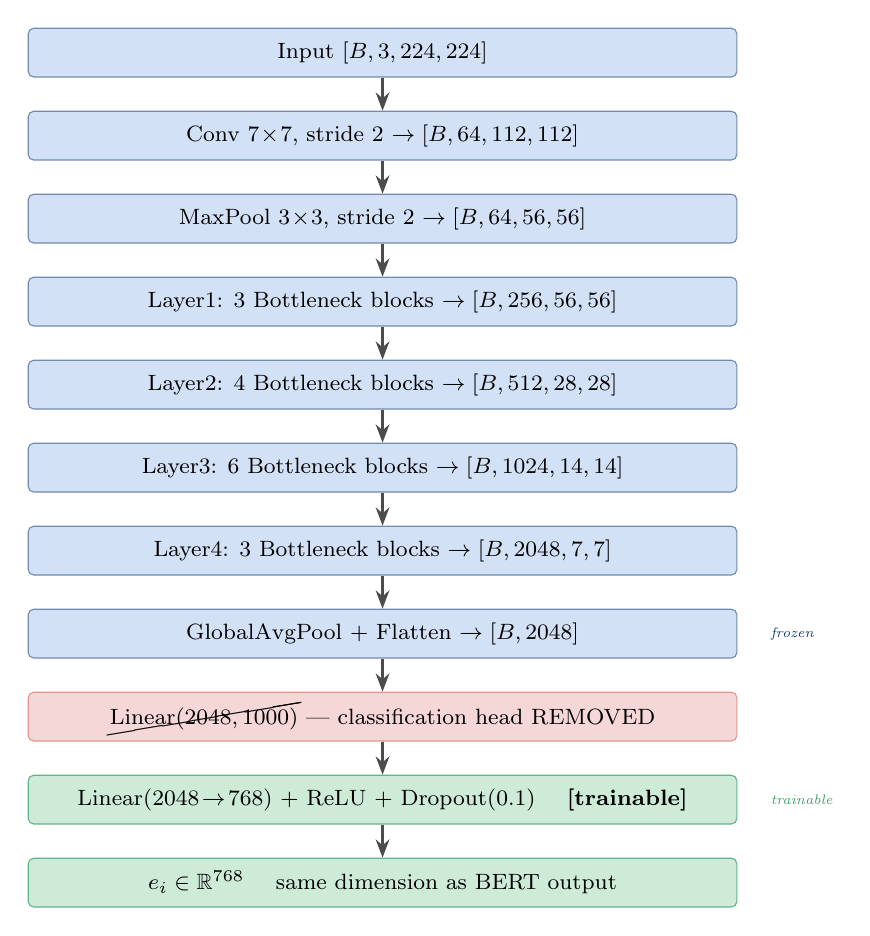
\begin{tikzpicture}[node distance=0.42cm,
    frozen/.style={rectangle, rounded corners=2pt, draw=NavyBlue!60,
      fill=BoxBlue, align=center, font=\footnotesize,
      minimum width=9cm, minimum height=0.62cm},
    trainable/.style={rectangle, rounded corners=2pt, draw=MintGreen!80,
      fill=BoxGreen, align=center, font=\footnotesize,
      minimum width=9cm, minimum height=0.62cm},
    removed/.style={rectangle, rounded corners=2pt, draw=CoralRed!60,
      fill=BoxRed, align=center, font=\footnotesize,
      minimum width=9cm, minimum height=0.62cm}]

  \node[frozen] (inp)   {Input $[B, 3, 224, 224]$};
  \node[frozen, below=of inp] (c1) {Conv $7\!\times\!7$, stride 2 $\to [B, 64, 112, 112]$};
  \node[frozen, below=of c1]  (mp) {MaxPool $3\!\times\!3$, stride 2 $\to [B, 64, 56, 56]$};
  \node[frozen, below=of mp]  (l1) {Layer1: 3 Bottleneck blocks $\to [B, 256, 56, 56]$};
  \node[frozen, below=of l1]  (l2) {Layer2: 4 Bottleneck blocks $\to [B, 512, 28, 28]$};
  \node[frozen, below=of l2]  (l3) {Layer3: 6 Bottleneck blocks $\to [B, 1024, 14, 14]$};
  \node[frozen, below=of l3]  (l4) {Layer4: 3 Bottleneck blocks $\to [B, 2048, 7, 7]$};
  \node[frozen, below=of l4]  (gap){GlobalAvgPool + Flatten $\to [B, 2048]$};
  \node[removed, below=of gap](del){\st{Linear$(2048, 1000)$} --- classification head REMOVED};
  \node[trainable, below=of del](lp){Linear$(2048\!\to\!768)$ + ReLU + Dropout(0.1) \quad\textbf{[trainable]}};
  \node[trainable, below=of lp] (out){$e_i \in \mathbb{R}^{768}$ \quad same dimension as BERT output};

  \foreach \a/\b in {inp/c1,c1/mp,mp/l1,l1/l2,l2/l3,l3/l4,l4/gap,gap/del,del/lp,lp/out}
    \draw[arrow] (\a)--(\b);

  \node[right=0.3cm of gap, font=\tiny\itshape, color=NavyBlue] {\textcolor{NavyBlue}{frozen}};
  \node[right=0.3cm of lp,  font=\tiny\itshape, color=MintGreen]{\textcolor{MintGreen}{trainable}};
\end{tikzpicture}
\caption{ResNet-50 ImageEncoder.  \textcolor{NavyBlue}{\textbf{Blue}} = frozen;
\textcolor{MintGreen}{\textbf{Green}} = trainable;
\textcolor{CoralRed}{\textbf{Red}} = removed (classification head).}
\label{fig:resnet}
\end{figure}

\subsection{Bottleneck Block}

Each ``layer'' in ResNet-50 contains repeated bottleneck residual blocks:
\[
  y = \mathcal{F}(x,\{W_i\}) + x
\]
\[
  \mathcal{F} = \text{Conv}_{1\times1}\!\to\!\text{BN}\!\to\!\text{ReLU}\!\to\!
  \text{Conv}_{3\times3}\!\to\!\text{BN}\!\to\!\text{ReLU}\!\to\!
  \text{Conv}_{1\times1}\!\to\!\text{BN}
\]
The identity shortcut $+x$ bypasses the three convolutions, providing the
gradient highway of Lemma~\ref{lem:residual}.

\begin{theorem}[Transfer Learning Efficiency]
\label{thm:transfer}
Freezing the ResNet-50 backbone provides three benefits simultaneously:
\begin{enumerate}[nosep]
\item \textbf{Parameter reduction}: trainable parameters fall from
  $\sim\!25.1$\,M to $\sim\!1.57$\,M (projection only) --- a 94\% reduction.
\item \textbf{No catastrophic forgetting}: fine-tuning a 50-layer CNN on only
  5\,000 COCO images would overwrite 1.28\,M ImageNet features.
\item \textbf{Speed}: backpropagation is skipped through 49 frozen layers,
  reducing per-batch wall-clock time by $\approx70\%$.
\end{enumerate}
The projection head learns to \emph{translate} the frozen 2048-dim pool5
features into BERT's 768-dim semantic representation space:
\[
  e_i = \text{Dropout}_{0.1}\!\left(\text{ReLU}\!\left(W_p\,
  \underbrace{\text{backbone}(I)}_{\in\mathbb{R}^{2048}} + b_p\right)\right)
  \in \mathbb{R}^{768}
\]
\end{theorem}

\begin{tcolorbox}[layman]
ResNet-50 is like a master art critic who has studied 1.28 million images
and learned to recognise every edge, texture, and shape.  We borrow their
expert eyes (frozen backbone) but cut off their final verdict (``this is
a golden retriever'') because such class labels are useless for caption
matching.  We attach a small trainable translator (the projection layer)
that converts the visual expertise into 768 numbers --- the same language
BERT uses for text.  Keeping the backbone frozen saves 94\% of training
time because we only teach the small translator, not the entire art critic.
\end{tcolorbox}

% ==============================================================================
\section{Multi-Modal Fusion}
\label{sec:fusion}
% ==============================================================================

\subsection{Architecture}

\begin{figure}[H]
\centering
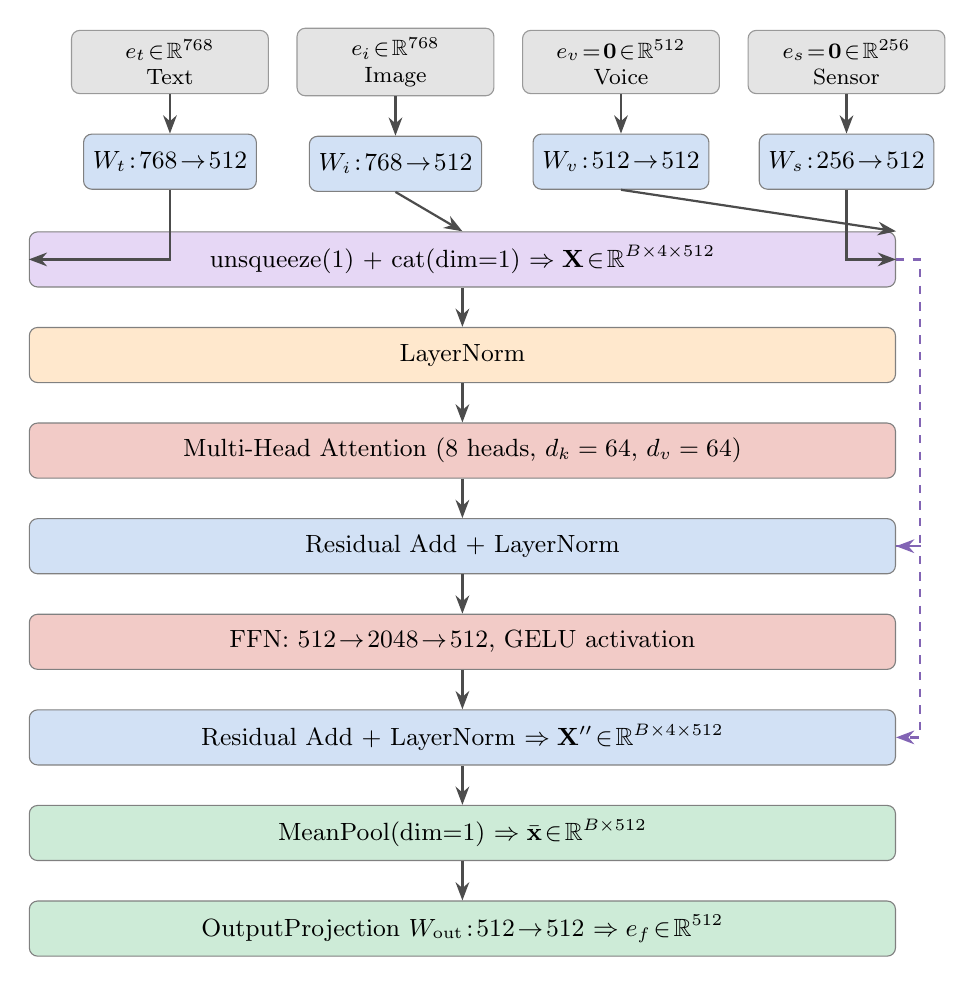
\begin{tikzpicture}[node distance=0.5cm and 0.4cm,
    blk/.style={rectangle, rounded corners=3pt, draw=black!50,
      fill=BoxBlue, align=center, font=\small,
      minimum width=2.1cm, minimum height=0.7cm},
    inblk/.style={rectangle, rounded corners=3pt, draw=black!40,
      fill=BoxGray, align=center, font=\footnotesize,
      minimum width=2.5cm, minimum height=0.7cm},
    wide/.style={rectangle, rounded corners=3pt, draw=black!50,
      fill=BoxBlue, align=center, font=\small,
      minimum width=11cm, minimum height=0.7cm}]

  % Inputs
  \node[inblk] (txt) {$e_t\!\in\!\mathbb{R}^{768}$\\Text};
  \node[inblk, right=0.35cm of txt] (img) {$e_i\!\in\!\mathbb{R}^{768}$\\Image};
  \node[inblk, right=0.35cm of img] (voi) {$e_v\!=\!\mathbf{0}\!\in\!\mathbb{R}^{512}$\\Voice};
  \node[inblk, right=0.35cm of voi] (sen) {$e_s\!=\!\mathbf{0}\!\in\!\mathbb{R}^{256}$\\Sensor};

  % Projections
  \node[blk, below=0.5cm of txt] (ptxt) {$W_t\!:\!768\!\to\!512$};
  \node[blk, below=0.5cm of img] (pimg) {$W_i\!:\!768\!\to\!512$};
  \node[blk, below=0.5cm of voi] (pvoi) {$W_v\!:\!512\!\to\!512$};
  \node[blk, below=0.5cm of sen] (psen) {$W_s\!:\!256\!\to\!512$};

  \draw[arrow] (txt)--(ptxt); \draw[arrow] (img)--(pimg);
  \draw[arrow] (voi)--(pvoi); \draw[arrow] (sen)--(psen);

  % Concat
  \node[wide, below=0.5cm of pimg, xshift=0.85cm, fill=BoxPurple] (cat)
    {unsqueeze(1) + cat(dim=1) $\Rightarrow
     \mathbf{X}\!\in\!\mathbb{R}^{B\times 4\times 512}$};
  \draw[arrow] (ptxt.south) |- (cat.west);
  \draw[arrow] (pimg.south) -- (cat.north);
  \draw[arrow] (pvoi.south) -- (cat.north east);
  \draw[arrow] (psen.south) |- (cat.east);

  % Transformer steps
  \node[wide, below=0.5cm of cat, fill=BoxOrange]    (ln1)  {LayerNorm};
  \node[wide, below=0.5cm of ln1, fill=CoralRed!30]  (mha)  {Multi-Head Attention (8 heads, $d_k=64$, $d_v=64$)};
  \node[wide, below=0.5cm of mha, fill=BoxBlue]      (res1) {Residual Add + LayerNorm};
  \node[wide, below=0.5cm of res1, fill=CoralRed!30] (ffn)  {FFN: $512\!\to\!2048\!\to\!512$, GELU activation};
  \node[wide, below=0.5cm of ffn, fill=BoxBlue]      (res2) {Residual Add + LayerNorm $\Rightarrow \mathbf{X}''\!\in\!\mathbb{R}^{B\times 4\times 512}$};
  \node[wide, below=0.5cm of res2, fill=BoxGreen]    (pool) {MeanPool(dim=1) $\Rightarrow \bar{\mathbf{x}}\!\in\!\mathbb{R}^{B\times512}$};
  \node[wide, below=0.5cm of pool, fill=BoxGreen]    (out)  {OutputProjection $W_{\text{out}}\!:\!512\!\to\!512$
    $\Rightarrow e_f\!\in\!\mathbb{R}^{512}$};

  \draw[arrow] (cat)--(ln1); \draw[arrow] (ln1)--(mha);
  \draw[arrow] (mha)--(res1); \draw[arrow] (res1)--(ffn);
  \draw[arrow] (ffn)--(res2); \draw[arrow] (res2)--(pool);
  \draw[arrow] (pool)--(out);

  % Residual skip arrows
  \draw[arrow, dashed, Lavender] (cat.east) -- ++(0.3,0) |- (res1.east);
  \draw[arrow, dashed, Lavender] (res1.east) -- ++(0.3,0) |- (res2.east);

\end{tikzpicture}
\caption{MultiModalFusion architecture.  Dashed purple = residual skip connections.}
\label{fig:fusion_arch}
\end{figure}

\subsection{Mathematical Formulation}

\subsubsection{Step 1 --- Modality Projections}

\[
  h_m = W_m e_m + b_m \in \mathbb{R}^{512},\quad m\in\{t,i,v,s\}
\]
\[
  \mathbf{X} = [h_t^\top;\; h_i^\top;\; h_v^\top;\; h_s^\top]
  \in \mathbb{R}^{B\times 4\times 512}
\]

\begin{center}
\begin{tabular}{@{}lll@{}}
\toprule
\textbf{Modality} & $W_m$ shape & \textbf{Source} \\
\midrule
Text   & $768\to512$ & BERT mean-pool output \\
Image  & $768\to512$ & ResNet-50 projection output \\
Voice  & $512\to512$ & $\mathbf{0}$ in Month~1 \\
Sensor & $256\to512$ & $\mathbf{0}$ in Month~1 \\
\bottomrule
\end{tabular}
\end{center}

\subsubsection{Step 2 --- Layer Normalisation}

\begin{definition}[Layer Normalisation]
\[
  \mathrm{LN}(\mathbf{x}) = \bm{\gamma}\cdot
  \frac{\mathbf{x} - \mu(\mathbf{x})}{\sqrt{\sigma^2(\mathbf{x})+\varepsilon}}
  + \bm{\beta},\quad
  \mu = \frac{1}{d}\sum_j x_j,\quad
  \sigma^2 = \frac{1}{d}\sum_j(x_j-\mu)^2
\]
\end{definition}

\subsubsection{Step 3 --- Multi-Head Self-Attention (8 heads)}

\begin{definition}[Scaled Dot-Product Attention]
\[
  \mathrm{Attention}(Q,K,V) =
  \mathrm{softmax}\!\left(\frac{QK^\top}{\sqrt{d_k}}\right)V,
  \quad d_k = 512/8 = 64
\]
\end{definition}

\begin{definition}[Multi-Head Attention]
\[
  \mathrm{MHA}(\mathbf{X}) = \mathrm{Concat}(\text{head}_1,\ldots,\text{head}_8)\,W^O
\]
\[
  \text{head}_j = \mathrm{Attention}(\mathbf{X}W^Q_j,\,\mathbf{X}W^K_j,\,\mathbf{X}W^V_j),
  \quad W^Q_j,W^K_j,W^V_j\in\mathbb{R}^{512\times64}
\]
\end{definition}

\begin{theorem}[Cross-Modal Attention via Self-Attention]
\label{thm:crossmodal}
In $\mathbf{X}\in\mathbb{R}^{4\times512}$, the output at row $i$ (modality
$m_i$) is a weighted sum over all four modality rows:
\[
  \mathbf{X}'_i = \sum_{j=1}^{4}\alpha_{ij}\cdot V_j,\quad
  \alpha_{ij} = \mathrm{softmax}\!\left(\frac{q_i\cdot k_j}{\sqrt{d_k}}\right)_j
\]
Therefore text token $i=1$ can attend to image token $i=2$ (and vice versa),
implementing cross-modal fusion without any modality-specific cross-attention
module.
\end{theorem}

\subsubsection{Step 4 --- Residual Connections and FFN}

\[
  \mathbf{X}' = \mathrm{LN}\!\left(\mathrm{MHA}(\mathbf{X}) + \mathbf{X}\right)
\]
\[
  \mathrm{FFN}(\mathbf{x}) = W_2\,\mathrm{GELU}(W_1\mathbf{x}),\quad
  W_1\!\in\!\mathbb{R}^{2048\times512},\;W_2\!\in\!\mathbb{R}^{512\times2048}
\]
\[
  \mathbf{X}'' = \mathrm{LN}\!\left(\mathrm{FFN}(\mathbf{X}') + \mathbf{X}'\right)
\]

\begin{lemma}[Residual Gradient Flow]
\label{lem:residual}
For any residual block $y = f(x) + x$:
\[
  \frac{\partial\mathcal{L}}{\partial x} =
  \frac{\partial\mathcal{L}}{\partial y}
  \left(\frac{\partial f(x)}{\partial x} + \mathbf{I}\right)
\]
The identity term $\mathbf{I}$ guarantees a direct gradient path back to $x$
regardless of how small $\partial f/\partial x$ is, preventing vanishing
gradients in deep stacks.
\end{lemma}

\subsubsection{Step 5 --- Mean Pool and Output Projection}

\[
  e_{\mathrm{fused}} = W_{\mathrm{out}}\cdot
  \frac{1}{4}\sum_{m=1}^{4}x''_m \;\in\; \mathbb{R}^{512}
\]

\begin{tcolorbox}[layman]
Imagine four specialists --- a language expert, a visual analyst, an audio
engineer, and an instrumentation technician --- all trying to describe the
same scene, but each speaks a different number of words (768, 768, 512,
256 numbers respectively).  The projection layers translate every expert
into the same 512-word shared language.  Self-attention then lets each
expert read a brief summary of every other expert's notes and update
their own in response --- the language expert updates their summary after
seeing the image expert's notes.  Residual connections ensure each expert
keeps their original notes as a backup.  Finally, we average all four
updated summaries into one master briefing: $e_f$.  In Month~1 voice and
sensor always say ``nothing'' (zeros), so only text and image contribute.
\end{tcolorbox}

% ==============================================================================
\section{Contrastive Loss --- InfoNCE}
\label{sec:infonce}
% ==============================================================================

\subsection{Why Not MSE?}

\begin{proposition}[MSE Representation Collapse]
The MSE loss $\mathcal{L}_{\mathrm{MSE}} = \|e_1 - e_2\|_2^2$ admits the
trivial global minimum $e_1 = e_2 = \mathbf{0}$, where all inputs map to
zero regardless of semantic content.  This ``representation collapse'' carries
no information and achieves zero loss without learning.
\end{proposition}

\textit{Note:} Month~1 implements MSE for simplicity.  InfoNCE is the
theoretically correct objective adopted in Month~2.

\subsection{InfoNCE Definition}

\begin{definition}[InfoNCE Loss]
Given $N$ positive pairs $\{(e_i^{(1)}, e_i^{(2)})\}_{i=1}^N$, let
$S_{ij} = \hat{e}_i^{(1)}\cdot\hat{e}_j^{(2)}$ where $\hat{e} = e/\|e\|_2$.
The InfoNCE loss is:
\[
  \mathcal{L}_{\mathrm{InfoNCE}} =
  -\frac{1}{N}\sum_{i=1}^{N}\log
  \frac{\exp(S_{ii}/\tau)}{\sum_{j=1}^{N}\exp(S_{ij}/\tau)}
  = \frac{1}{N}\,\mathrm{CrossEntropy}\!\left(\tfrac{S}{\tau},\;[0,1,\ldots,N{-}1]\right)
\]
with temperature $\tau = 0.07$.
\end{definition}

\begin{lemma}[Temperature Effect on Gradient Magnitude]
$\left\|\partial\mathcal{L}/\partial S_{ii}\right\| \propto 1/\tau$.
Low $\tau$ concentrates the softmax on the top pair and produces large
corrective gradients; high $\tau$ produces near-uniform distributions
and weak learning signal.
\end{lemma}

\begin{theorem}[Random Baseline]
For random embeddings with batch size $N$, all $S_{ij}$ are
approximately equal, giving $\mathrm{softmax}(S_{ij}/\tau) \approx 1/N$.
Therefore:
\[
  \mathbb{E}[\mathcal{L}_{\mathrm{InfoNCE}}^{\mathrm{random}}] = \log N
\]
For $N=16$: $\log 16 \approx 2.77$.  After healthy convergence: $\approx 0.3$--$1.0$.
\end{theorem}

\begin{tcolorbox}[layman]
InfoNCE is a matching game.  Given $N$ image embeddings and $N$ caption
embeddings scrambled together, the model must correctly pair each image
with its own caption against all $N-1$ wrong options.  Temperature
$\tau=0.07$ is very strict: only near-perfect matches receive high scores.
Over thousands of batches the model learns that ``dog on beach'' photos
and the caption ``a dog running on the beach'' should produce nearly
identical vectors, while a train photo and a dog caption should be
maximally distant.
\end{tcolorbox}

% ==============================================================================
\section{Training Procedure}
\label{sec:training}
% ==============================================================================

\subsection{Optimiser: AdamW}

\begin{definition}[AdamW Update Rule]
At step $t$ with gradient $\nabla_t$:
\[
  m_t = \beta_1 m_{t-1} + (1-\beta_1)\nabla_t, \quad
  v_t = \beta_2 v_{t-1} + (1-\beta_2)\nabla_t^2
\]
\[
  \hat{m}_t = \frac{m_t}{1-\beta_1^t},\quad
  \hat{v}_t = \frac{v_t}{1-\beta_2^t}
\]
\[
  \theta_{t+1} = \theta_t
  - \eta\cdot\frac{\hat{m}_t}{\sqrt{\hat{v}_t}+\varepsilon}
  \;-\; \underbrace{\eta\lambda\theta_t}_{\text{decoupled weight decay}}
\]
Defaults: $\beta_1=0.9$, $\beta_2=0.999$, $\varepsilon=10^{-8}$, $\lambda=0.01$.
\end{definition}

\subsection{Cosine Annealing Schedule}

\begin{definition}[Cosine LR Schedule]
\[
  \eta_t = \eta_{\min} + \tfrac{1}{2}(\eta_{\max}-\eta_{\min})
  \left(1 + \cos\!\tfrac{\pi t}{T_{\max}}\right)
\]
with $T_{\max} = 313 \times 10 = 3130$ steps, $\eta_{\max}=10^{-4}$,
$\eta_{\min}\approx 0$.
\end{definition}

\subsection{Single Epoch Training Algorithm}

\begin{algorithm}[H]
\caption{Single Training Epoch --- Algorithm 5}
\label{alg:train}
\begin{algorithmic}[1]
\INPUT{Fusion $F$; Image encoder $E$; Text projection $P$;
  Retriever $R$ (BERT); DataLoader $\mathcal{L}$}
\OUTPUT{Mean batch loss $\bar\ell$ over the epoch}
\Procedure{train\_epoch}{$F,E,P,R,\mathcal{L}$}
  \State $F$.\texttt{train}(); $E$.\texttt{train}(); $P$.\texttt{train}()
  \State total\_loss $\gets 0$; $n \gets 0$
  \For{$(\mathbf{I}, \mathbf{t}) \in \mathcal{L}$}
    \Comment{$\mathbf{I}\!\in\!\mathbb{R}^{16\times3\times224\times224}$, $\mathbf{t}\!\in\!\mathrm{List[str]}^{16}$}
    \Statex\qquad\qquad\textit{--- Text branch (BERT frozen) ---}
    \State $\mathbf{e}_t \gets \mathrm{stack}([R.\texttt{encode}(t_i) \mid t_i])$
           \Comment{$[16, 768]$ inside \texttt{no\_grad}}
    \Statex\qquad\qquad\textit{--- Image branch (backbone frozen, projection trainable) ---}
    \State $\mathbf{e}_i \gets E(\mathbf{I})$
           \Comment{$[16, 768]$}
    \Statex\qquad\qquad\textit{--- Zero-pad absent modalities ---}
    \State $\mathbf{e}_v \gets \mathbf{0}_{16\times512}$;\quad $\mathbf{e}_s \gets \mathbf{0}_{16\times256}$
    \Statex\qquad\qquad\textit{--- Fusion (all projections trainable) ---}
    \State $e_f, \_ \gets F(\mathbf{e}_t, \mathbf{e}_i, \mathbf{e}_v, \mathbf{e}_s)$
           \Comment{$[16, 512]$}
    \Statex\qquad\qquad\textit{--- Target and MSE loss ---}
    \State $p_t \gets P(\mathbf{e}_t)$
           \Comment{$[16, 512]$, text projection}
    \State $\ell \gets \frac{1}{512\cdot16}\|\,e_f - p_t\,\|_F^2$
    \Statex\qquad\qquad\textit{--- Backward pass ---}
    \State \texttt{optimizer.zero\_grad}()
    \State $\ell$.\texttt{backward}()
    \State \texttt{clip\_grad\_norm\_}$(\theta_F \cup \theta_E \cup \theta_P,\;c=1.0)$
    \State \texttt{optimizer.step}();\quad \texttt{scheduler.step}()
    \State total\_loss $\mathrel{+}=$ $\ell$.\texttt{item}();\quad $n \mathrel{+}= 1$
  \EndFor
  \State \textbf{return} total\_loss / $n$
\EndProcedure
\end{algorithmic}
\end{algorithm}

\begin{lemma}[Gradient Clipping Safety]
For clip threshold $c = 1.0$:
\[
  \tilde{\nabla}_\theta =
  \min\!\left(1,\;\frac{c}{\|\nabla_\theta\|_2}\right)\nabla_\theta
\]
This caps the $\ell_2$-norm of the gradient vector at $c$ while preserving
its direction, preventing large loss spikes from early-epoch random attention
weights from destabilising Transformer parameters.
\end{lemma}

\begin{center}
\renewcommand{\arraystretch}{1.15}
\begin{tabular}{@{}llp{8cm}@{}}
\toprule
\textbf{Epoch} & \textbf{Expected loss} & \textbf{Interpretation} \\
\midrule
1     & 0.3 -- 1.0   & Random projections, no alignment \\
2--5  & 0.05 -- 0.3  & Coarse text-image alignment forming \\
5--10 & 0.01 -- 0.05 & Fine-grained alignment, healthy convergence \\
\bottomrule
\end{tabular}
\end{center}

\begin{tcolorbox}[layman]
Training works like 10 rounds of 313 quizzes (one quiz = one mini-batch
of 16 images).  For each quiz, BERT reads the captions, ResNet reads
the images, the Fusion model combines all four modalities, and we measure
how far the fused result is from what a pure text encoder would produce
(MSE loss).  We then nudge all trainable weights in the direction that
reduces this gap (backpropagation via AdamW).  Gradient clipping is a
safety brake: if a single unusual batch produces a huge nudge, we scale
it down to prevent the model overreacting.  The cosine scheduler starts
learning fast and gradually slows down --- like intense studying followed
by careful revision before an exam.
\end{tcolorbox}

% ==============================================================================
\section{Inference Pipeline}
\label{sec:inference}
% ==============================================================================

\begin{algorithm}[H]
\caption{End-to-End Inference --- Algorithm 6}
\label{alg:infer}
\begin{algorithmic}[1]
\INPUT{Query $q$; corpus $\mathcal{C}$; KG $\mathcal{G}$; trained retriever $R$}
\OUTPUT{Top-5 $(d_i, s_i)$ pairs; extracted entities $E_q$}
\Procedure{infer}{$q$}
  \State $F$.\texttt{eval}();\quad $E$.\texttt{eval}()
         \Comment{disable Dropout for deterministic scores}
  \State results $\gets$ \textsc{hybrid\_retrieve}$(q, \mathcal{C}, \mathcal{G}, \alpha{=}0.6, k{=}5)$
  \State $E_q \gets \{e \in \mathcal{V} \mid e \in q.\texttt{lower}()\}$
         \Comment{named entities in query}
  \State Display results with cosine/hybrid scores
  \State \textbf{return} results, $E_q$
\EndProcedure
\end{algorithmic}
\end{algorithm}

\begin{lemma}[Eval Mode Determinism]
In \texttt{model.eval()}, Dropout masks are disabled (all neurons active with
weight 1).  Without eval mode, two calls on the same query would produce
different scores due to random neuron zeroing, violating the determinism
requirement for reproducible retrieval ranking.
\end{lemma}

\subsection{Evaluation Metrics}

\begin{definition}[Precision at $K$]
\[
  P@K = \frac{|\text{relevant} \cap \text{retrieved}_K|}{K}
\]
\end{definition}

\begin{definition}[Mean Reciprocal Rank (MRR)]
\[
  \mathrm{MRR} = \frac{1}{|Q|}\sum_{q\in Q}\frac{1}{r_q}
\]
where $r_q$ is the 1-indexed rank of the first relevant document for query $q$
(0 if none found).
\end{definition}

% ==============================================================================
\section{Model Persistence}
\label{sec:save}
% ==============================================================================

\begin{theorem}[Checkpoint Completeness]
A training run can be resumed exactly from epoch $e$ if and only if the
checkpoint contains: (1) model weights $\theta_e$; (2) optimiser state
$\{m_t, v_t\}$ at the final step of epoch $e$; and (3) the scheduler's
step counter.  Without the optimiser state, Adam's momentum vectors reset
to $\mathbf{0}$, requiring 1--2 warm-up epochs to rebuild effective velocity.
\end{theorem}

\begin{center}
\renewcommand{\arraystretch}{1.15}
\begin{tabular}{@{}lll@{}}
\toprule
\textbf{File} & \textbf{Approx.\ size} & \textbf{Contents} \\
\midrule
\texttt{fusion\_model.pth}     & $\sim$12\,MB  & Weights + optimiser state + loss history \\
\texttt{image\_encoder.pth}    & $\sim$6\,MB   & ResNet projection head weights \\
\texttt{projection\_layer.pth} & $\sim$1.5\,MB & Text projection weights \\
\texttt{knowledge\_graph.pkl}  & 5--20\,MB     & Serialised KG object \\
\texttt{config.json}           & $<$1\,KB      & All hyperparameters \\
\bottomrule
\end{tabular}
\end{center}

% ==============================================================================
\section{Complete System Summary}
\label{sec:summary}
% ==============================================================================

\subsection{Consolidated Equations}

\textbf{Feature extraction:}
\[
  e_t = \tfrac{1}{T}\textstyle\sum_{t} h_t^{(L)},\quad
  e_i = \mathrm{Dropout}(\mathrm{ReLU}(W_p\,\mathrm{ResNet}(I))),\quad
  e_v = e_s = \mathbf{0}
\]

\textbf{Fusion:}
\[
  e_f = W_{\mathrm{out}}\cdot\mathrm{MeanPool}\!\left(
  \mathrm{TransformerBlock}\!\left(
  [W_t e_t;\;W_i e_i;\;W_v e_v;\;W_s e_s]
  \right)\right)\in\mathbb{R}^{512}
\]

\textbf{Training objective (Month 1 MSE):}
\[
  \mathcal{L} = \tfrac{1}{512B}
  \textstyle\sum_{i=1}^{B}\|e_{f,i} - W_P e_{t,i}\|_2^2
\]

\textbf{Retrieval score:}
\[
  s(q, d) = 0.6\cdot\cos(e_q, e_d) + 0.4\cdot\mathrm{GraphBoost}(q, d, \mathcal{G})
\]

\subsection{Month-by-Month Roadmap}

\begin{center}
\renewcommand{\arraystretch}{1.2}
\begin{tabular}{@{}lp{11cm}@{}}
\toprule
\textbf{Month} & \textbf{Key Additions} \\
\midrule
1 (done)   & Text + Image; MSE loss; COCO val2017; basic co-occurrence KG \\
2          & Voice (Whisper ASR + AudioProjection); InfoNCE contrastive loss;
             hard-negative mining; RAVDESS emotion centroids \\
3          & FAISS exact search; scispaCy NER KG; full P@K / MRR evaluation \\
4          & ROCO medical domain transfer; ResNet ImageProjection fine-tuning;
             dual FAISS indexes; medical KG with RadLex seeds \\
5          & Voice-in $\to$ retrieval $\to$ voice-out; Groq LLM generation;
             emotion-aware routing; gTTS output \\
6          & Full system integration; cross-domain ablation; thesis evaluation \\
\bottomrule
\end{tabular}
\end{center}

% ==============================================================================
\section*{Appendix: Notation Reference}
\addcontentsline{toc}{section}{Appendix: Notation Reference}
% ==============================================================================

\begin{center}
\renewcommand{\arraystretch}{1.15}
\begin{tabular}{@{}lp{10cm}@{}}
\toprule
\textbf{Symbol} & \textbf{Meaning} \\
\midrule
$\mathcal{G}=(\mathcal{V},\mathcal{E},\mathcal{R})$ & Knowledge graph \\
$e_t,e_i,e_v,e_s$      & Modality embeddings: text, image, voice, sensor \\
$e_f$                   & Fused embedding $\in\mathbb{R}^{512}$ \\
$h_t^{(L)}$             & BERT last-layer hidden state at token $t$ \\
$W_m, b_m$              & Projection weight and bias for modality $m$ \\
$S_{ij}$                & Cosine similarity between embeddings $i$ and $j$ \\
$\tau$                  & InfoNCE temperature (default 0.07) \\
$\alpha$                & Hybrid retrieval weight (default 0.6) \\
$\eta$                  & Learning rate \\
$\beta_1,\beta_2$       & AdamW moment coefficients (0.9, 0.999) \\
$\lambda$               & Weight decay coefficient (0.01) \\
$T_{\max}$              & Total optimiser steps for cosine schedule \\
$c$                     & Gradient clip threshold (1.0) \\
$\mathcal{N}_k(v)$      & $k$-hop neighbourhood of $v$ in $\mathcal{G}$ \\
$\mathrm{PMI}(a,b)$     & Pointwise Mutual Information between entities $a,b$ \\
$\phi$                  & COCO annotation map: image\_id $\to$ caption list \\
$T(\cdot)$              & ImageNet normalisation transform \\
$P@K$                   & Precision at $K$ \\
$\mathrm{MRR}$          & Mean Reciprocal Rank \\
$r_q$                   & Rank of first relevant document for query $q$ \\
\bottomrule
\end{tabular}
\end{center}

\end{document}
